\phantomsection
\section*{BUỔI 1: CẤU HÌNH EXPRESS}
\addcontentsline{toc}{section}{\numberline{}Buổi 1: Cấu Hình Express}
\setcounter{section}{1}
% =========================================================
% \clearpage
\phantomsection
\subsection*{Bước 0: Cài đặt Node và Git}
\addcontentsline{toc}{subsection}{\numberline{}Bước 0: Cài đặt node và git}
\setcounter{subsection}{1}
\setcounter{figure}{0}
\begin{figure}[H]
  \centering
  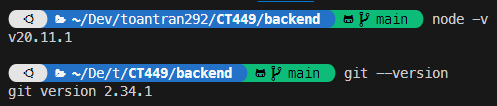
\includegraphics{images/chapterFirst/1.png}
  \caption{\bfseries Phiên bản của node và git}
\end{figure}
% =========================================================
\phantomsection
\subsection*{Bước 1: Tạo ứng dụng Node}
\addcontentsline{toc}{subsection}{\numberline{}Bước 1: Tạo ứng dụng node}
\setcounter{subsection}{2}
\setcounter{figure}{0}
\begin{figure}[H]
  \centering
  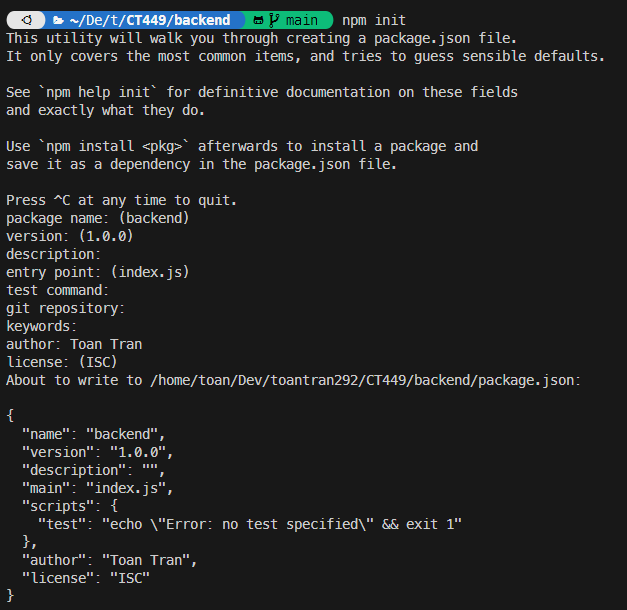
\includegraphics[width=15cm]{images/chapterFirst/2.png}
  \caption{\bfseries Tạo file package.json}
\end{figure}
\begin{figure}[H]
  \centering
  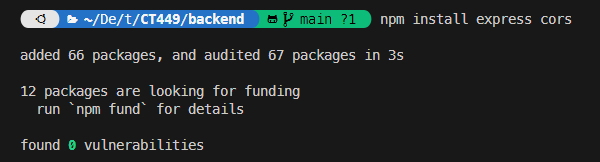
\includegraphics{images/chapterFirst/3.png}
  \caption{\bfseries Cài đặt các package}
\end{figure}
% =========================================================
\phantomsection
\subsection*{Bước 2: Quản lý mã nguồn dự án với Git và Github}
\addcontentsline{toc}{subsection}{\numberline{}Bước 2: Quản lý mã nguồn dự án với git và github}
\setcounter{subsection}{3}
\setcounter{figure}{0}
\begin{figure}[H]
  \centering
  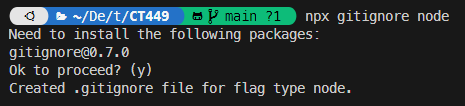
\includegraphics{images/chapterFirst/4.png}
  \caption{\bfseries Tạo file .gitignore}
\end{figure}
\begin{figure}[H]
  \centering
  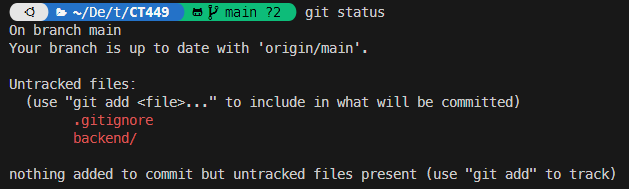
\includegraphics[width=15cm]{images/chapterFirst/5.png}
  \caption{\bfseries Khi chạy câu lệnh "git status"}
\end{figure}
\begin{figure}[H]
  \centering
  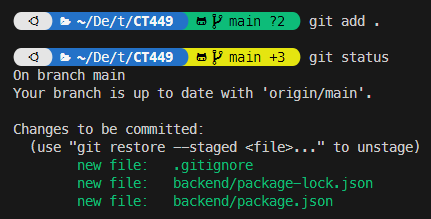
\includegraphics{images/chapterFirst/6.png}
  \caption{\bfseries Thêm các file vào chuẩn bị commit}
\end{figure}
\begin{figure}[H]
  \centering
  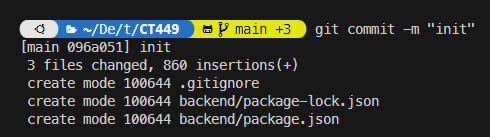
\includegraphics{images/chapterFirst/7.png}
  \caption{\bfseries Commit các file}
\end{figure}
% =========================================================
\phantomsection
\subsection*{Bước 3: Cài đặt Express}
\addcontentsline{toc}{subsection}{\numberline{}Bước 3: Cài đặt express}
\setcounter{subsection}{3}
\setcounter{figure}{0}
\begin{figure}[H]
  \centering
  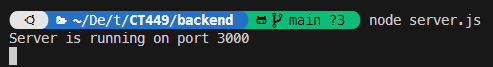
\includegraphics{images/chapterFirst/8.png}
  \caption{\bfseries Khởi chạy server}
\end{figure}
\begin{figure}[H]
  \centering
  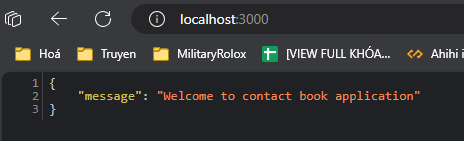
\includegraphics{images/chapterFirst/9.png}
  \caption{\bfseries Thử API bằng cách truy cập bằng trình duyệt}
\end{figure}
\begin{figure}[H]
  \centering
  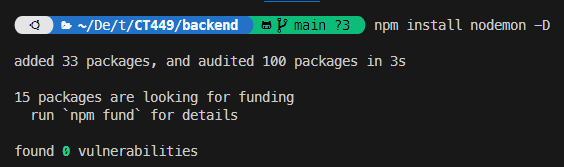
\includegraphics{images/chapterFirst/10.png}
  \caption{\bfseries Cài đặt nodemon}
\end{figure}
\begin{figure}[H]
  \centering
  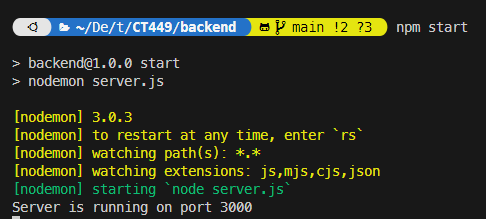
\includegraphics{images/chapterFirst/11.png}
  \caption{\bfseries Chạy server bằng script start}
\end{figure}
\begin{figure}[H]
  \centering
  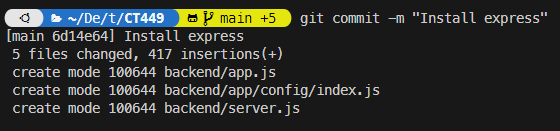
\includegraphics{images/chapterFirst/12.png}
  \caption{\bfseries Commit cài đặt express}
\end{figure}
% =========================================================
\phantomsection
\subsection*{Bước 4: Định nghĩa Controller và Route}
\addcontentsline{toc}{subsection}{\numberline{}Bước 4: Định nghĩa controller và route}
\setcounter{subsection}{4}
\setcounter{figure}{0}
\begin{figure}[H]
  \centering
  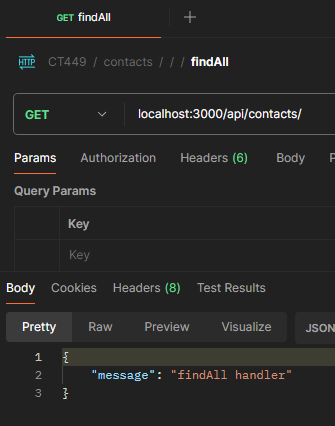
\includegraphics[width=8cm]{images/chapterFirst/13.png}
  \caption{\bfseries Thử API find all contacts bằng postman}
\end{figure}
\begin{figure}[H]
  \centering
  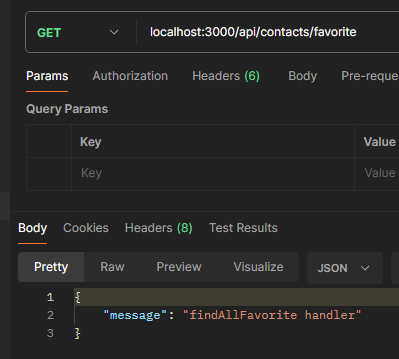
\includegraphics{images/chapterFirst/14.png}
  \caption{\bfseries Thử API find all contact favorites bằng postman}
\end{figure}
\begin{figure}[H]
  \centering
  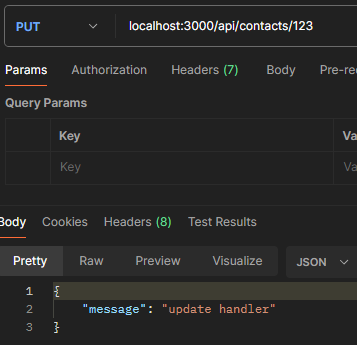
\includegraphics{images/chapterFirst/15.png}
  \caption{\bfseries Thử API update contact favorites bằng postman}
\end{figure}
% =========================================================
\phantomsection
\subsection*{Bước 5: Cài đặt xử lý lỗi}
\addcontentsline{toc}{subsection}{\numberline{}Bước 5: Cài đặt xử lý lỗi}
\setcounter{subsection}{5}
\setcounter{figure}{0}
\begin{figure}[H]
  \centering
  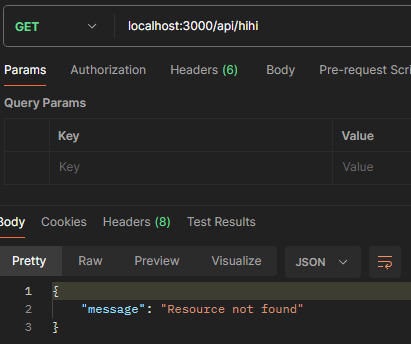
\includegraphics{images/chapterFirst/16.png}
  \caption{\bfseries Thử API lỗi bằng postman}
\end{figure}